% !TEX root =  master.tex
\chapter{Projektphase 1 – Firewall}
Die Firewall-Konfigurationen wurden mittels IP-Tables auf der Opfermaschine erstellt. Dabei wurden Bash-Scripts implementiert, um die jeweils notwendigen Befehle nachvollziehen zu können. Zudem wird sämtlicher Datenverkehr der Penetrationstests aufgezeichnet und interpretiert. 

\section{Offene Konfiguration}

Zunächst wird auf der Opfermaschine eine offene Konfiguration der Firewall erstellt. Das bedeutet in diesem Fall, dass jeglicher eingehender sowie jeglicher ausgehender Datenverkehr ungehindert zugelassen wird. In dieser Konfiguration werden weder Kommunikationsquellen noch Inhalt gefiltert oder geblockt.

\subsection{Script}
Der erste Schritt setzt die IP-Tables auf ihre Ursprungswerte zurück. Das heißt, dass alle einkommenden, ausgehenden und weitergeleiteten Pakete ungefiltert zugelassen werden. Zusätzlich zu der normalen IP-Tables Konfiguration wird hier auch noch die NAT-Konfiguration gesetzt.  
Das Script besteht aus drei wesentlichen Prozessen: 
\begin{itemize}
	\item Einstellung der Regeln (inklusive NAT)
	\item Flushing der Regeln
	\item Logging
\end{itemize} 

Als nächstes werden alle noch überbleibenden Ausnahmeregelungen `geflushed`. Das bedeutet, dass diese gelöscht und auf den Standardwert zurückgesetzt werden. Hierdurch wird eine saubere und reproduzierbare Basiskonfiguration sichergestellt.\\
Abschließend wird das Logging behandelt. Damit am Ende des Vorgangs nachvollzogen werden kann, welche Pakete eingetroffen bzw. ausgetreten sind, wird der Datenverkehr vom Script aus protokolliert.
Zusätzlich zu den drei Funktionen des Scripts wird nach Abschluss die Konfiguration in der Konsole ausgegeben.

\newpage

\lstinputlisting[language=bash]{scripts/firewall-open.sh}

\newpage
Output: 
\lstinputlisting[]{scripts/output_firewall-open.sh}

\subsection{Penetrationtest – Inward}
Da nun die Firewall der Opfermaschine konfiguriert wurde, können Penetrationstests durchgeführt werden. 
Zunächst wird geprüft, welche Informationen über einen Portscan mit NMAP herausgefunden werden können. 
Während der laufenden Scans wird zusätzlich der Datenverkehr der Opfermaschine mit Hilfe von Wireshark aufgezeichnet. 
Dies hilft dabei die Reaktion – bzw. das Fehlen einer Reaktion – der Opfermaschine nachzuvollziehen.
\subsubsection{nmap 10.0.2.4 -p- -A -T4}
Der erste NMAP-Scan wird mit vier paramentern versehen. Zunächst muss die Zieladresse des Opfers angegeben werden. In diesem Fall befindet sich das Opfer im NAT-Netzwerk an der Adresse 10.0.2.4. Als nächstes wird die gewünschte Menge der Ports angegeben. Standardmäßig werden die 1000 wichtigsten Ports geprüft. Auf Grund der Gründlichkeit dieses Tests werden jedoch alle 65.535 Ports der Opfermaschine gescannt – zu erkennen am Parameter -p-. Darauf folgend wird erneut ein Parameter zu Gunsten der Gründlichkeit gesetzt. Der Parameter -A setzt die Aggressivität des Scans. So werden durch diesen Parameter Funktionen wie OS-Detection, Version-Scanning, Script-Scanning und Traceroute verwendet. Zuletzt wird ein Geschwindigkeitsparameter gesetzt. \\

Output:
\lstinputlisting[]{scripts/scans/nmap_p_A_T4}

Im Output ist zu erkennen, dass alle gescannten Ports geschlossen sind. Dies war zu erwarten, da auf der Opfermaschine keine Services laufen und somit keine Ports genutzt werden. Dennoch lässt der Fakt, dass die Ports als geschlossen gezeigt werden, auf weitere Informationen schließen. Zum einen wird dadurch bekannt, dass die Anfragen ungefiltert an die Opfermaschine durchgekommen sind. Im gleichen Zuge wird erkannt, dass die Angreifermaschine Antworten auf ihre Anfragen erhalten hat. Demnach kann der Angreifer zu dem Entschluss kommen, dass die Firewall offen ist. 
Zusätzlich zu dem Portstatus wird die MAC-Adresse und der Hersteller des Geräts identifiziert. Zudem versucht das Tool Angaben über das Betriebssystem zu machen. In diesem Fall konnte kein Betriebssystem identifiziert werden, da die Antworten zu ungenau bzw. zu generisch waren. Als letzte Information gibt NMAP die Traceroute an. Das heißt, es wird angegeben welchem Pfad die Anfragen gefolgt sind und wie lange sie für den Rundentrip gebraucht haben.

\begin{figure}
	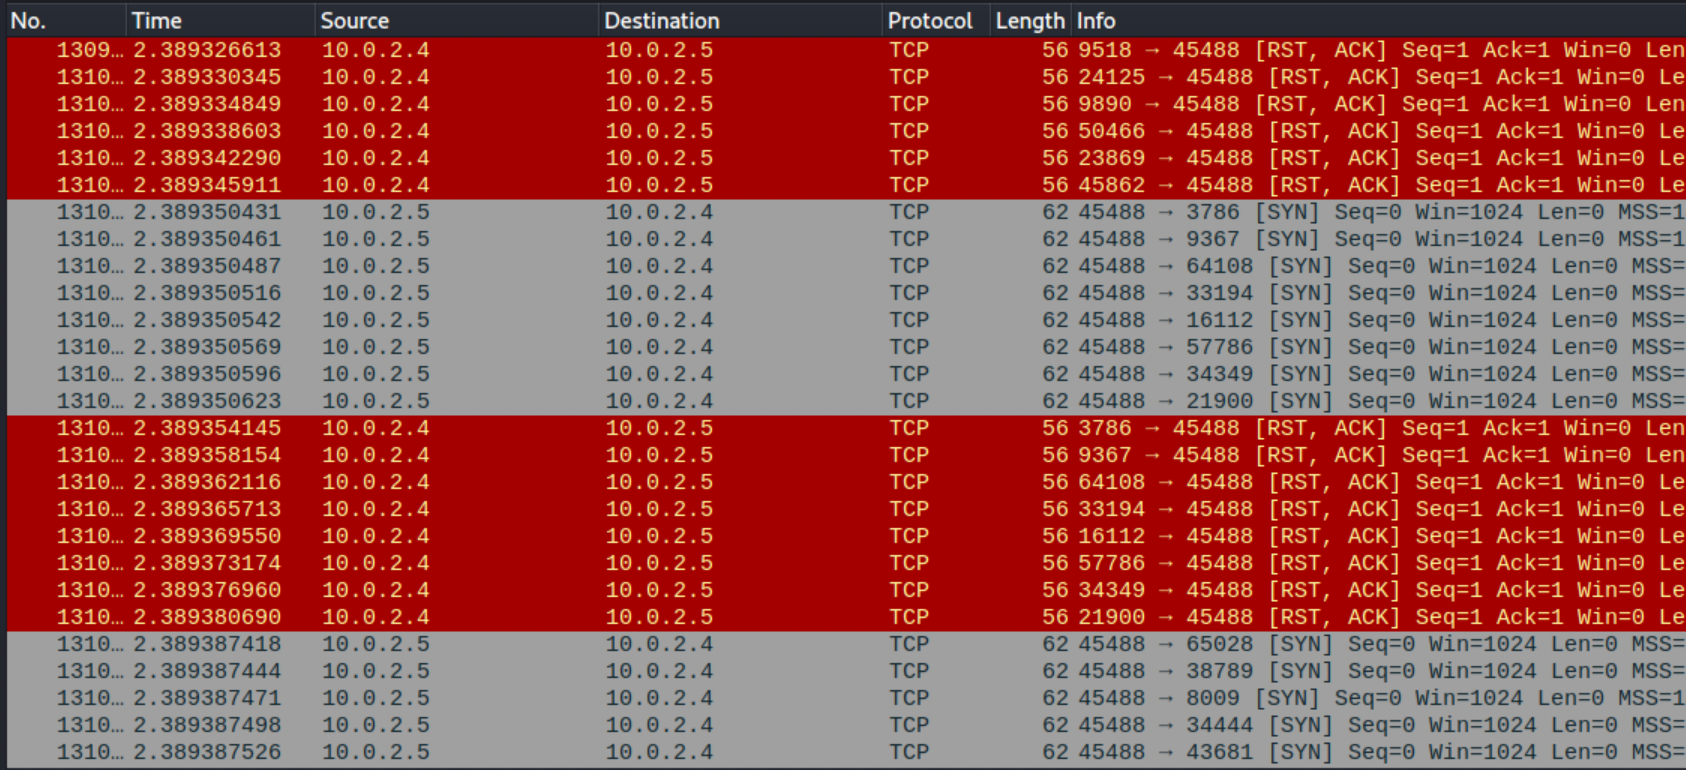
\includegraphics[width=\linewidth]{img/ws_firewall-open.png}
	\caption{Datenverkehr bei offener Firewall}
	\label{fig:ws_firewall_open}
\end{figure}

Im Wireshark-Mitschnitt (Abbildung \ref{fig:ws_firewall_open}) wird der Datenverkehr der Opfermaschine gezeigt. Zu erkennen in grau, sind die eingehenden Anfragen der Angreifermaschine. Hier werden TCP SYN Anfragen an das Opfer geschickt und eine ACK bzw. RST Antwort erwartet. Dies ist die Einleitung einer TCP Verbindung, welche bei diesem Scan nie vollständig durchgeführt wird. Da die Ports der Opfermaschine nicht gefiltert werden, werden die Anfragen verarbeitet und dem Angreifer wird geantwortet. Bei Eingang einer ACK oder RST Nachricht auf der Angreifermaschine wird der Kontakt zum Port abgebrochen und somit keine Verbindung erstellt. Alleine durch das Antworten verrät das Opfer bereits den Status der Ports. Sollte der Angreifer eine ACK Nachricht erhalten, so ist der gefragte Port offen und "hört" auf einkommende Anfragen. Im Falle einer RST Nachricht ist der Port geschlossen.
 Sollte keine Antwort verschickt werden interpretiert NMAP den Port als gefiltert. Ein SYN Scan eignet sich besonders aufgrund der Geschwindigkeit des Scans und der Verlässlichkeit der Ergebnisse.

\subsubsection{nmap 10.0.2.4 -sU -T4}
 Zu prüfen, ob die Verbindung via UDP ebenfalls offen ist, wird als nächster Schritt ein UDP Scan mit NMAP durchgeführt. Wie bei dem vorherigen Scan sind hier ebenfalls die Parameter für die Geschwindigkeit gesetzt. Der -A Parameter wurde gegen -sU ausgetauscht. Der -sU Parameter gibt den Scantyp an. So wird anstatt eines TCP SYN Scans ein UDP Scan durchgeführt. Obwohl TCP den Großteil des Internetverkehrs prägt, ist UDP kein zu vernachlässigendes Protokoll. Bei diesem Scan werden UDP Pakete an die Ports geschickt. NMAP erwartet im Gegenzug ICMP Antworten. Entweder die Opfermaschine schickt eine Nachricht, dass der gewünschte Port nicht erreichbar ist – Port ist geschlossen – oder es wird eine andere Errornachricht verschickt, in welchem Falle der Port als gefiltert gesehen wird. Sollte das Opfer eine UDP Antwort verschicken, so ist der Port offen. Sei es der Fall, dass der Angreifer keine Antwort erhält wird der Port als entweder offen oder gefiltert interpretiert. 
Ein großes Hindernis an UDP Scanning ist der Zeitaufwand, da NMAP bei offenen Ports keine Antwort erhält und daraufhin auf den Timeout warten muss. Auf Grund dessen werden bei diesem Scan nur die wichtigsten 1000 Ports gescannt. Zudem ist die Verbindung via UDP wesentlich unverlässlicher als über TCP, was zu verfälschten Ergebnissen führen kann.

\begin{figure}
	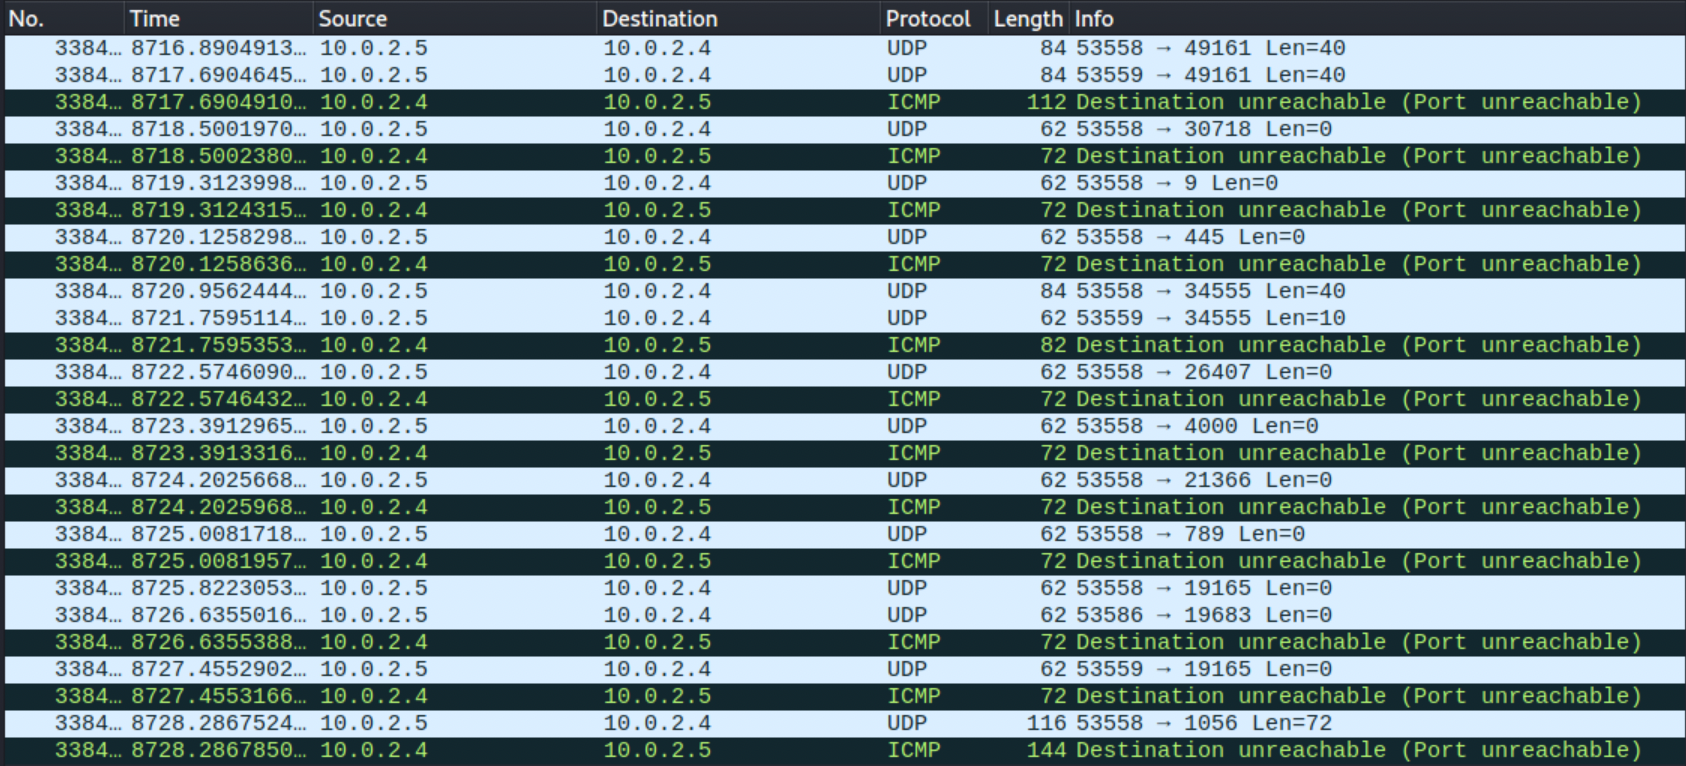
\includegraphics[width=\linewidth]{img/ws_firewall_open_udp.png}
	\caption{Datenverkehr bei offener Firewall – UDP}
	\label{fig:ws_firewall_open_udp}
\end{figure}

Auf der Abbildung \ref{fig:ws_firewall_open_udp} ist zu erkennen, wie der UDP Scan verläuft. Wie bereits beschrieben werden der Opfermaschine UDP Pakete geschickt (zu sehen in Blau). Darauf folgt die Antwort des Opfers – in diesem Fall als ICMP Error – dass der gewünschte Port nicht zu erreichen ist. Aus diesem Grund interpretiert NMAP die Ports der Opfermaschine als geschlossen. \newpage

\lstinputlisting{scripts/scans/nmap_sU_T4}

Am Output des Scans lässt sich erkennen, dass dieser wesentlich länger gebraucht hat als der vorherige TCP Scan. So hat der UDP Scan 18 Minuten gebraucht um die wichtigesten 1000 Ports des Opfers zu scannen. Desweiteren wird berichtet, dass acht Ports offen bzw. gefiltert sind. Da keine Services auf der Opfermaschine laufen oder Firewall-Filter gesetzt sind lässt sich vermuten, dass diese Ports fehlerhaft als offen | gefiltert angezeigt werden. So kann es sein, dass die Opfermaschine nicht schnell genug auf die Anfragen des Angreifers geantwortet haben und somit der Timeout von NMAP erreicht wurde. 

\subsection{Penetrationtest - Outward}
Als nächstes wird getestet, welchen Einfluss die Firewall auf die Funktionalität der Maschine hat. Es werden hierbei zwei Punkte getestet. Zunächst wird mittels wget überprüft, ob das World-Wide-Web erreichbar ist. Daraufhin wird überprüft, ob andere Maschinen im Netzwerk erreicht werden können. 

\subsubsection*{wget https://google.com}

Um zu testen ob das WWW von der Opfermaschine erreichbar ist, wurde mittels des wget Befehls versucht google.com zu erreichen. Das Ziel war es eine index.html von Google zu erhalten und dadurch zu verdeutlichen, dass sowohl HTTPS wie auch DNS auf der Maschine uneingeschränkt funktionieren. Da in dieser Firewall-Konfiguration alle Ports uneingeschränkt sind war davon auszugehen, dass die Maschine ohne Fehler eine index.html erhalten sollte. \\
\begin{figure}
	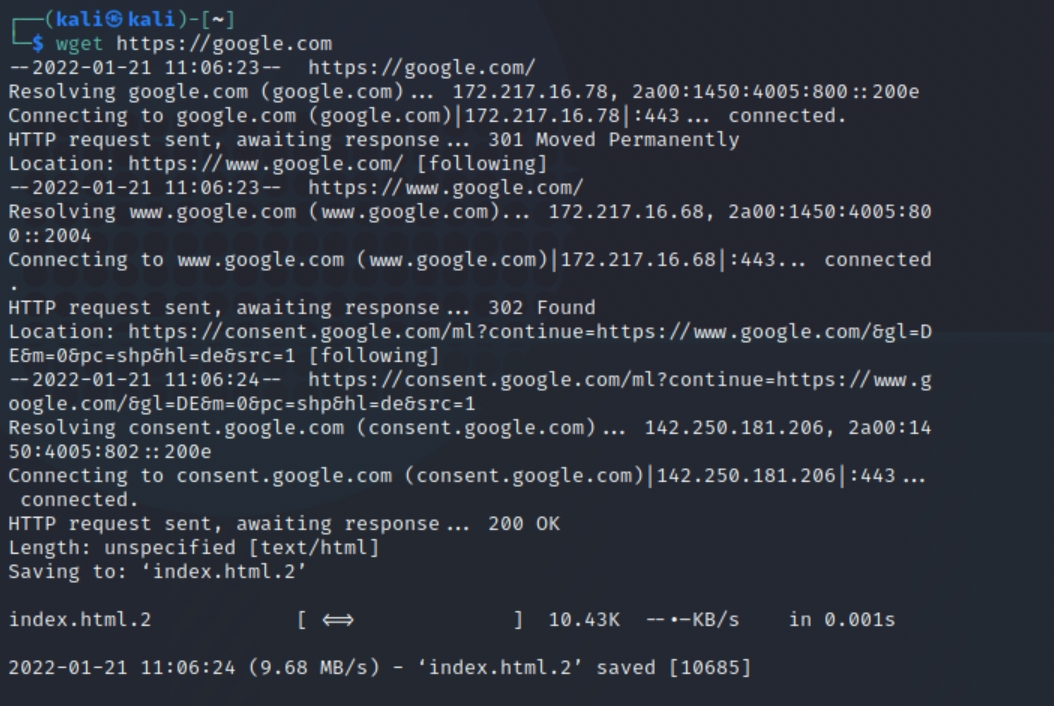
\includegraphics[width=\linewidth]{img/open-in-out-output.png}
	\caption{wget bei offener Firewall-Konfiguration}
	\label{fig:wget_open}
\end{figure}

Wie im Output \ref*{fig:wget_open} zu erkennen, wird auf Anfrage eine index.html von https://google.com erhalten. Demnach lässt sich erkennen, dass sowohl HTTPS wie auch DNS funktionieren. 

\subsubsection*{nc 10.0.2.5 4445}
Als nächstes wurde überprüft, ob eine Verbindung zu einer benachbarten Maschine hergestellt werden kann. Um dies zu testen, wurde über das Tool NetCat versucht eine Verbindung auf dem Port 4445 der Zielmaschine herzustellen. Damit eine Verbindung hergestellt werden kann, wurde auf der Maschine 10.0.2.5 im Terminal der komplementäre Befehl ``nc -lvp 4445 -e /bin/bash' ausgeführt. So weiß die Zielmaschine, auf welchem Port nach Verbindungsanfragen gelauscht werden muss. Zusätzlich erhält der Kommunikationspartner Zugriff auf Konsolenfunktionen der Zielmaschine. So kann nach Verbindungsaufbau kontrolliert werden, dass die Verbindung erstellt wurde. 
\begin{figure}
	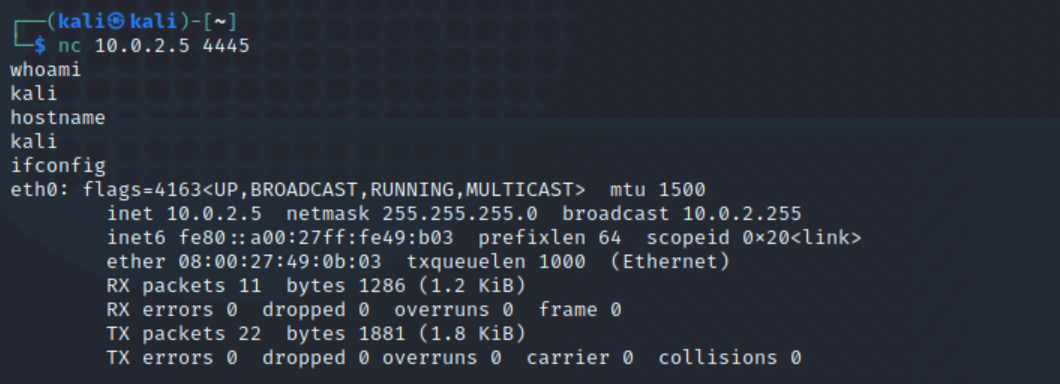
\includegraphics[width=\linewidth]{img/open_nc.png}
	\caption{NetCat-Ergebnis bei offener Konfiguration}
	\label{fig:nc_open}
\end{figure}
\\Im Output \ref{fig:nc_open} lässt sich erkennen, dass die Maschine 10.0.2.4 nun Zugriff auf die Konsole der Maschine 10.0.2.5 besitzt. Durch den Befehl ifconfig, lässt sich dies beweisen. Demnach hat die Verbindung funktioniert, was bei dieser offenen Konfiguration zu erwarten war. 
\section{Geschlossene Konfiguration}
Als nächstes wird eine Konfiguration getestet, in der alle Verbindungen geblockt werden. Zu dieser Konfiguration gehören die Ausnahmen: SSH und localhost. Das Ziel dieses Tests ist es zu prüfen, wie die Opfermaschine von außen angesprochen werden kann – bzw. welche Informationen ein potentieller Angreifer erhalten könnte.
 
\subsection{Script}
Dieses Script besteht aus sechs Teilen: 
\begin{itemize}
	\item Flushing der Regeln
	\item Ausnahmeregelungen
	\item Standardregelungen
	\item Localhost
	\item Bestehende Verbindungen
	\item Logging
\end{itemize}
Zunächst werden alle bestehenden Regeln gelöscht. Dies geschieht wie in dem vorherigen Script mit Hilfe des Flushingbefehls. Darauf folgen die Ausnahmeregelungen. Diese werden hier als nächstes gesetzt, da die Reihenfolge der Regeln bei den IP-Tables durchaus einen Einfluss hat. In diesem Fall wird der Port 22 freigegeben. Sowohl eintreffende wie auch ausgehende Nachrichten dürfen über den Port 22 gehandhabt werden. Dies erlaubt es mit der Virtual Machine eine SSH Verbindung aufzubauen. \\
Um dann die Firewall so einzustellen, dass keine weiteren Verbindungen zugelassen werden, werden nun die Standardregelungen gesetzt. Im Gegenzug zum vorherigen Script werden nun die eingehenden, ausgehenden und weitergeleiteten Verbindungen "gedroppt". So werden alle Pakete die über die betroffenen Ports laufen fallen gelassen und nicht bearbeitet. \\
Damit trotzdessen der localhost weiterhin funktioniert, werden noch einmal Ausnahmen beschrieben.
Zusätzlich werden bestehende Verbindungen weiterhin zugelassen, um keine laufenden Prozesse zu stören. Somit kann gesichert sein, dass plötzliche Änderungen in der Firewall keine Probleme in der Anwendung mitsichziehen. 
Abschließend werden erneut die Loggingbefehle gesetzt.

\newpage

\lstinputlisting[language=bash]{scripts/firewall-closed.sh}

\newpage

\lstinputlisting{scripts/output_firewall-closed}

\subsection{Penetrationtest – Inward}
Nun sind alle Ports der Opfermaschine geblockt bzw. gefiltert. Um zu überprüfen, ob das Script funktioniert hat werden nun eine Reihe an Tests abgeschlossen. Zunächst werden wieder NMAP Scans die Grundlage bilden, von der wichtige Informationen über das Ziel abgeleitet werden können.

\subsubsection{nmap 10.0.2.4 -p- -A -T4}
Es wird nun erneut mittels eines TCP SYN Scans geprüft, welche Ports des Opfers offen sind. Zu Gunsten der Genauigkeit und der Vergleichbarkeit des Scans wurde die Konfiguration der Parameter aus dem Kapitel 2.1.2 übernommen.
Ebenfalls wird erneut der Datenverkehr der Opfermaschine aufgezeichnet. 
\newpage
\lstinputlisting{scripts/scans/nmap_p_A_T4_closed}

An der Ausgabe des Scans lässt sich erkennen, dass trotz der verschärften Regelungen die MAC Adresse sowie der Hersteller des Geräts erkannt wurde. 
Der wichtigste Punkt ist jedoch, dass alle Ports des Opfers nun als gefiltert anstatt als geschlossen erkannt werden. Dies liegt daran, dass keine Antwort auf die SYN Pakete des Angreifers verschickt werden. Wie bereits beschrieben, interpretiert NMAP bei einem TCP SYN Scan das Fehlen einer Antwort als Filterung des angesprochenen Ports. Dies wird anhand der Abbildung \ref{fig:ws_firewall_closed} deutlich. Dort ist zu sehen, wie die Pakete der Angreifermaschine von der Adresse 10.0.2.5 auf der Opfermaschine eintreffen. Jedoch antwortet die Opfermaschine nicht, anders als in Abbildung \ref{fig:ws_firewall_open}.

\begin{figure}
	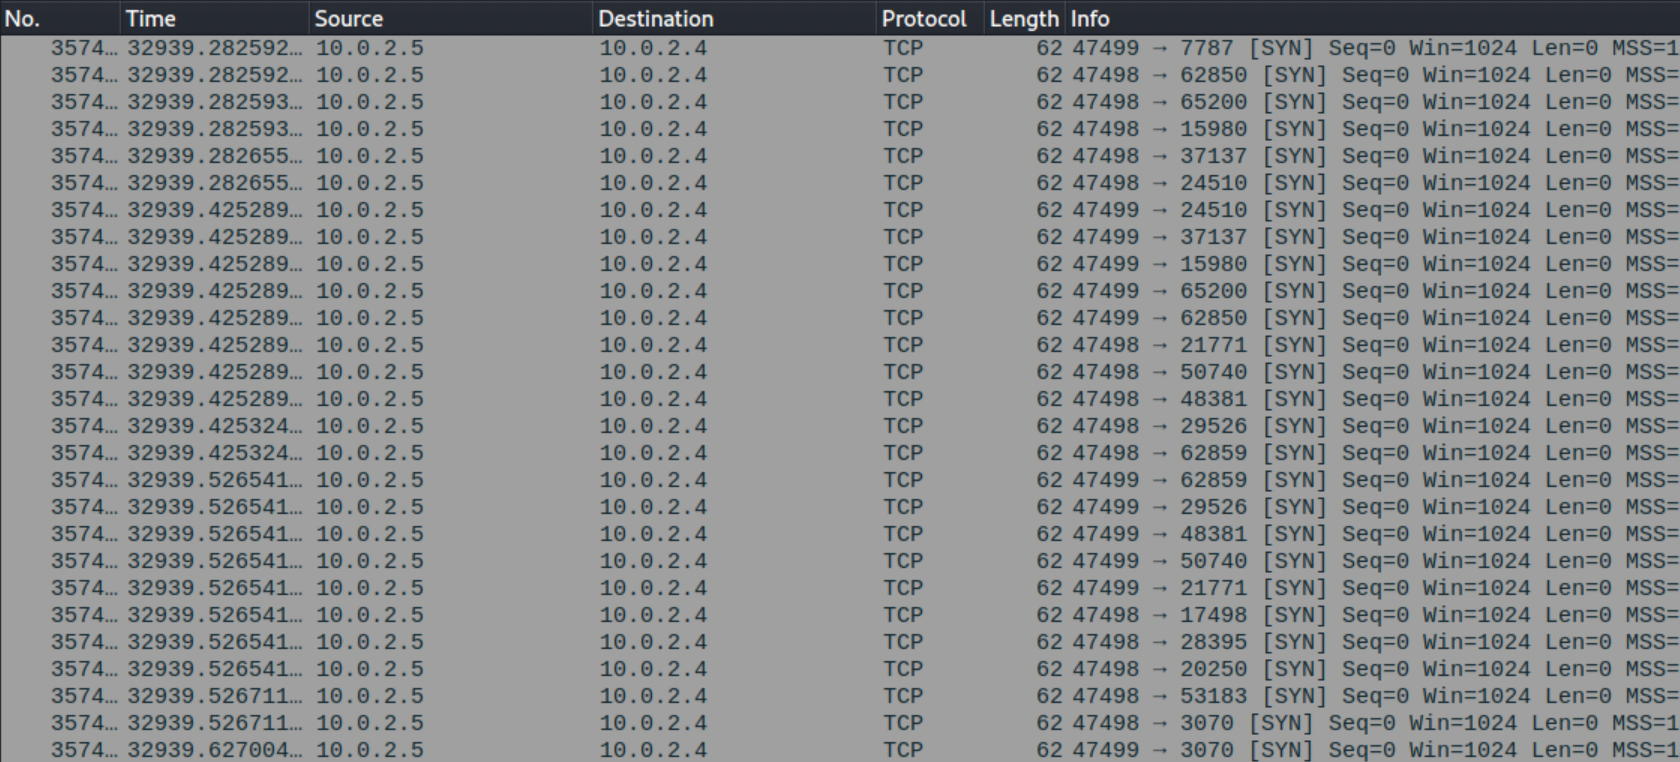
\includegraphics[width=\linewidth]{img/ws_firewall_closed.png}
	\caption{Datenverkehr bei geschlossener Firewall}
	\label{fig:ws_firewall_closed}
\end{figure}

\subsubsection{nmap 10.0.2.4 -sU -T4}
Um zu Prüfen, welchen Einfluss das Script auf UDP Pakete nimmt, wird als nächstes ein UDP Scan durchgeführt. Wie auch beim vorherigen Scan, bleiben die Parameter gleich. Die Erwartung an dieses Scanergebnis ist, dass alle Ports der Opfermaschine als offen | gefiltert angezeigt werden. Zudem wird erwartet, dass dieser Scan wesentlich mehr Zeit in Anspruch nimmt, als der Scan aus dem Kapitel 2.1.2. Diese Erwartungshaltung bildet sich aus der Art und Weise, wie der UDP Scan funktioniert. Da die Ports des Opfers durch das Bash-Script geschlossen sein sollten, sollten keine Antwortpakete an den Angreifer geschickt werden. Somit müsste der Angreifer auf den Timeout von NMAP warten, welcher zur gleichen Zeit die Ports als offen bzw. gefiltert interpretiert.

\begin{figure}
	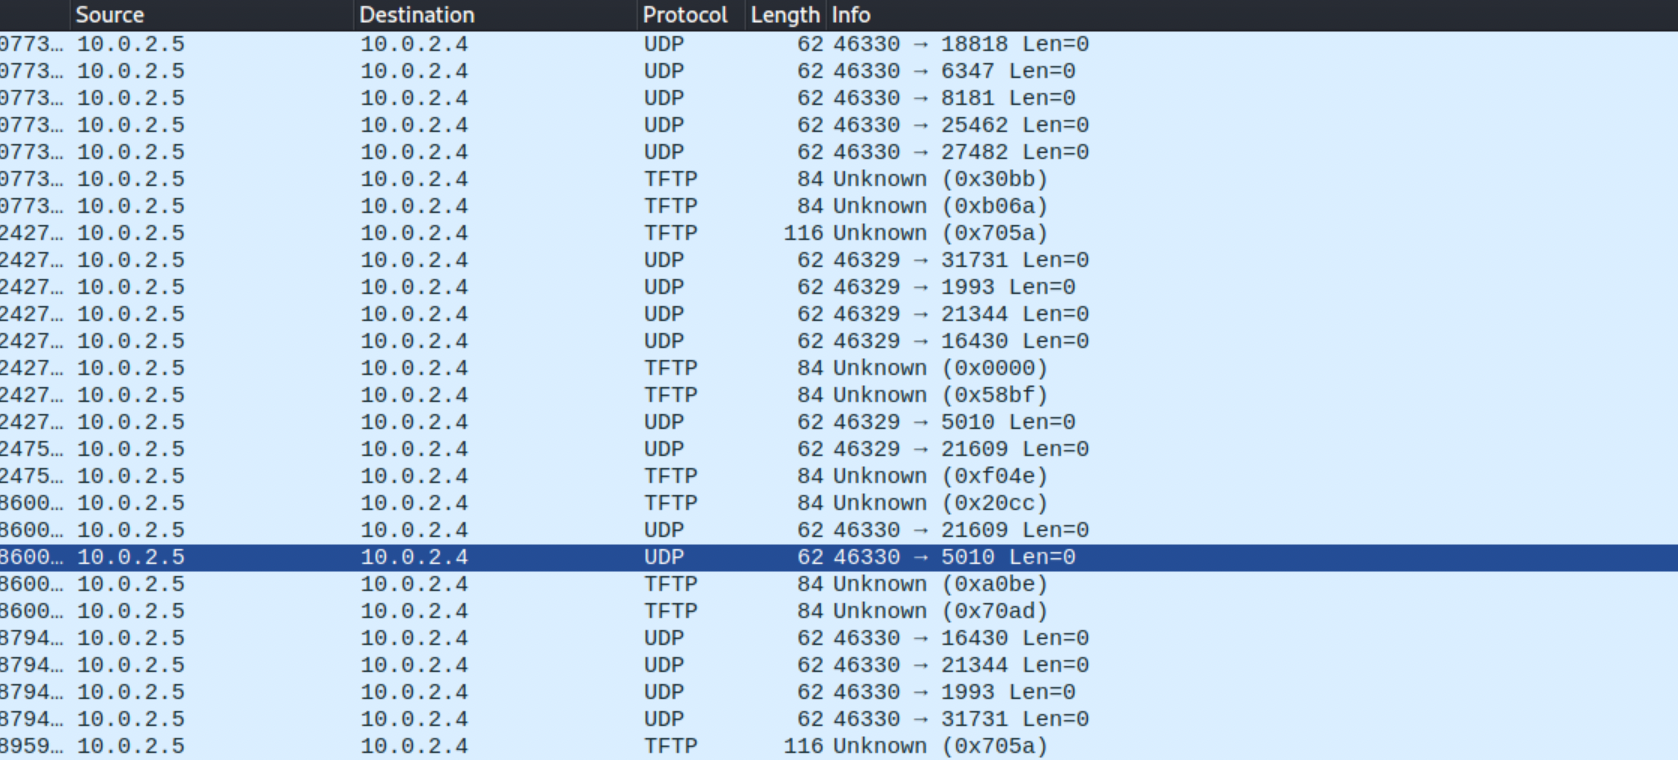
\includegraphics[width=\linewidth]{img/ws_firewall_closed_udp.png}
	\caption{Datenverkehr bei geschlossener Firewall – UDP}
	\label{fig:ws_firewall_closed_udp}
\end{figure}
Output:
\lstinputlisting{scripts/scans/nmap_sU_T4_closed}

Der Output bestätigt die Hypothese. Da der Angreifer keine Antworten erhalten hat, kann keine genaue Aussage über den Status der Ports getroffen werden. 

\subsection{Penetrationtest – Outward}
Wie auch bei der vorherigen Konfiguration, wird gestestet welchen Einfluss die Firewall auf die Funktionstüchtigkeit der Maschine hat. 
Da sowohl eingehende als auch ausgehende Verbindungen von der Firewall geblockt werden, ist es anzunehmen, dass beide Tests fehlschlagen.

\subsubsection*{wget https://google.com}
Zunächst wird erneut getestet, ob das WWW von der Maschine zu erreichen ist. Dafür wird versucht eine index.html von google.com zu erhalten. Da der Port 443 – für https – geblockt ist, ist zu erwarten, dass die Verbindung fehlschlägt. Zudem ist Port 53 – welcher für DNS zuständig ist – ebenfalls geblockt. Was dazu führt, dass der Name google.com keiner IP zugeordnet werden kann. Um zusätzlich zu überprüfen, ob der tatsächliche Server von Google ebenfalls nicht erreichbar ist, wird die IP direkt genutzt. 

\begin{figure}
	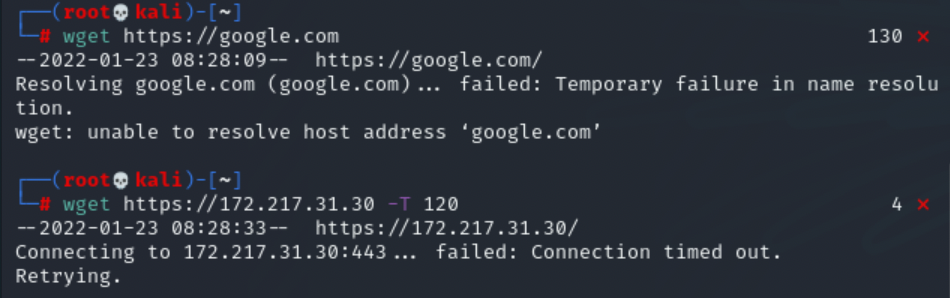
\includegraphics[width=\linewidth]{img/closed-in-out-output.png}
	\caption{Versuch eines Verbindungsaufbaus bei geschlossener Firewall}
	\label{fig:closed_in_out}
\end{figure}

Wie im Output \ref*{fig:closed_in_out} zu erkennen, lässt sich weder über DNS noch über eine direkte IP Adresse eine Verbindung zu google.com aufbauen. Demnach ist es bewiesen, dass die Firewall keine Verbindung ins World Wide Web zulässt.

\subsubsection*{nc 10.0.2.5 4445}

Als nächstes wird getestet, ob die Maschine sich mit einer benachbarten Maschine via NetCat verbinden kann. Da alle Ports geblockt sind, ist zu erwarten, dass keine Verbindung hergestellt werden kann. Das Vorgehen ist das Gleiche, wie im Kapitel 2.1.3.
Zunächst wird auf der Nachbarmaschine – 10.0.2.5 – der Port 4445 mittels NetCat geöffnet und darauf gewartet, dass eine Verbindung hergestellt wird. Daraufhin wird auf der Maschine 10.0.2.4 mittels des NetCat Befehls versucht eine Verbindung aufzubauen. Um zu erkennen, wann eine Verbindung fehlschlägt, wird dem Befehl der Modifier -w angehängt. Dieser erlaubt es eine Sekundenzahl als Timeout anzugeben.
Output:
\lstinputlisting{scripts/nc_closed}
Wie zu erkennen, lässt sich keine Verbindung zu Nachbarmaschine herstellen. Dies war zu erwarten, da alle Ports von der Firewall blockiert werden.

\newpage
\section{Standard Konfiguration}

\lstinputlisting[language=bash]{scripts/firewall-standard.sh}

\subsection{Script}
Das Script zur Erstellung einer Firewall, wie sie möglicherweise in Unternehmen vorkommen könnte, ähnelt dem aus Kapitel 2.2.1 sehr. 
Es besteht aus den gleichen sechs Teilen, obwohl das Logging hier auf Grund der Länge des Scripts vernachlässigt wird.
Zunächst werden alle bestehenden Regeln gelöscht – gefluscht – um die Firewall auf ihre Basiskonfiguration zurückzusetzen. Dies verhindert mögliche Konflikte mit bestehenden Regeln im weiteren Verlauf. \\
Darauf folgend werden alle eingehenden, weiterleitenden und ausgehenden Verbindungen blockiert, bestehende Verbindungen sowie Antworten auf Etablierte werden jedoch weiterhin zugelassen. 
Abschließend werden die Ausnahmeregelungen behandelt, welche den Hauptunterschied zu der vorherigen Konfiguration darstellen. \\
Hier werden die Ports für SSH sowohl eingehend als auch ausgehend zugelassen. Zusätzlich werden die Ports 22, 53, 80 und 443 ausgehend zugelassen, hauptsächlich um Verbindung zum Internet herstellen zu können. 
Zudem sind dem Port 53 UDP Verbindungen gestattet, da das DNS Protokoll hauptsächlich über UDP funktioniert. 

\subsection{Penetrationstest – Inward}
\subsubsection{nmap 10.0.2.4 -p- -A -T4}
Wie auch bei den vorherigen Konfigurationen, wird hier ebenfalls zunächst ein TCP SYN Scan durchgeführt. Da in dieser Firewall-Konfiguration keine fundamentalen Veränderungen durchgeführt wurden, werden den Vorgängern ähnliche Ergebnisse erwartet. Es sollte der Angreifermaschine nur ein Port ersichtlich sein, da alle Anderen nur von innen nach außen funktionieren. \\
Output:
\begin{figure}
	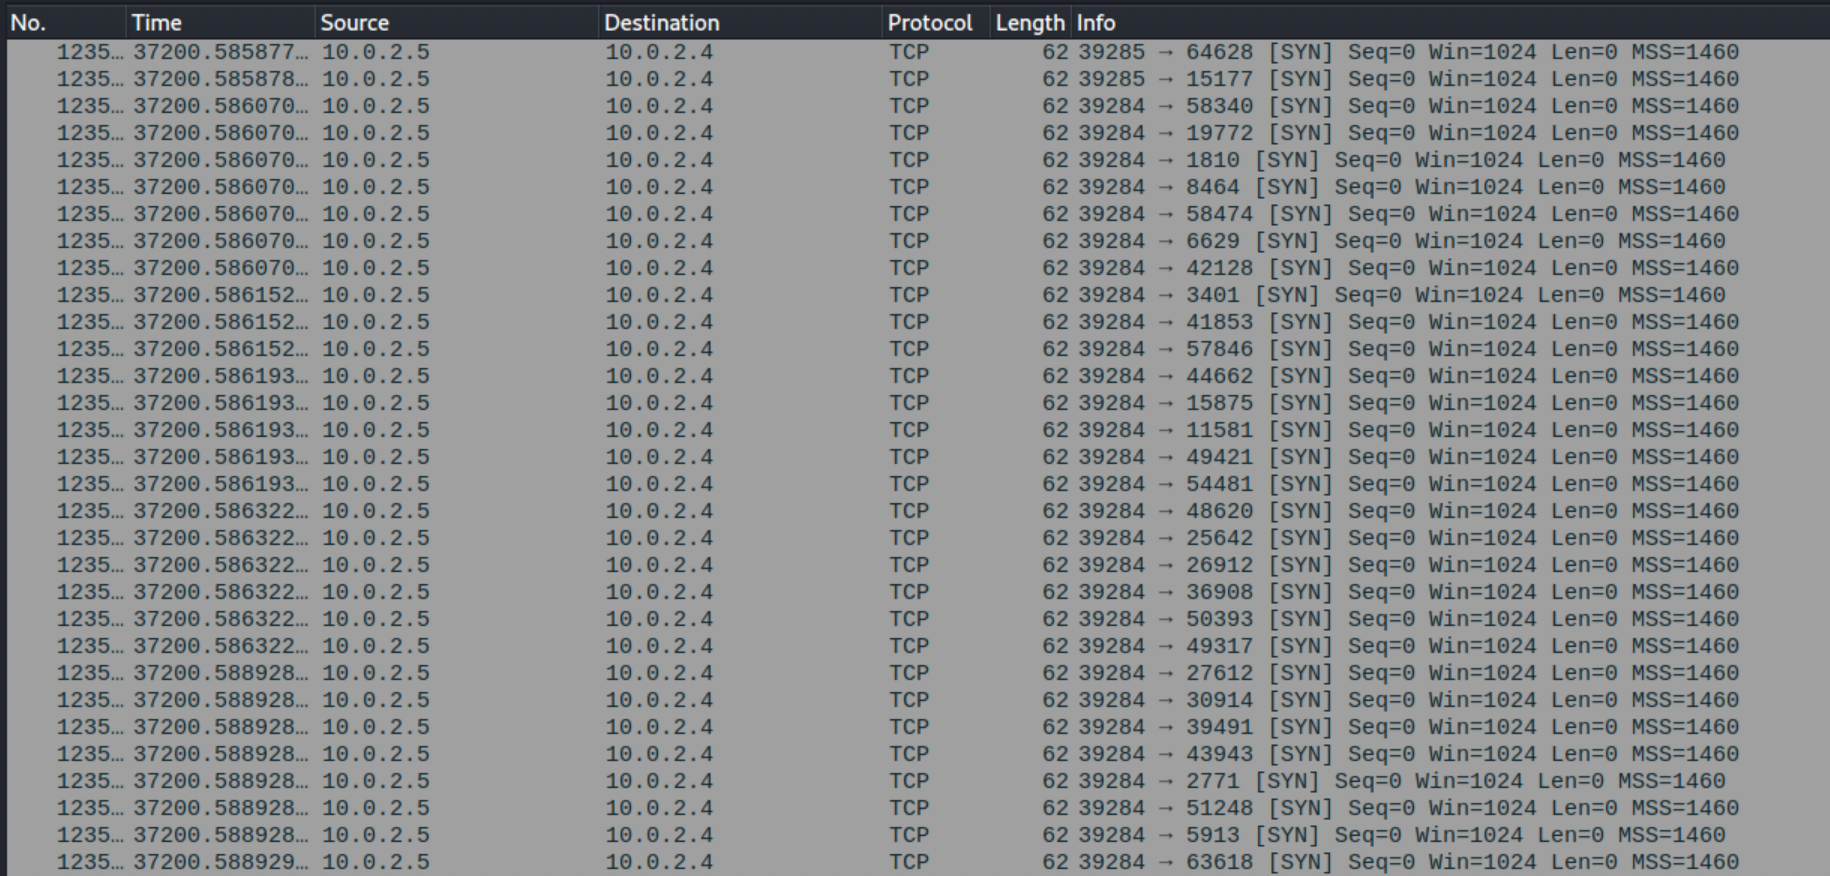
\includegraphics[width=\linewidth]{img/ws_firewall_standard.png}
	\caption{Datenverkehr der Opfermaschine}
	\label{fig:ws_firewall_standard}
\end{figure}

\lstinputlisting{scripts/scans/nmap_p_A_T4_standard}

Der Output dieses Scans ist identisch mit dem aus Kapitel 2.2.2, mit der Ausnahme des Ports 22. Ein maßgeblicher Unterschied wird sich erst bei einem ausgehenden Test erkennen lassen.

\begin{figure}
	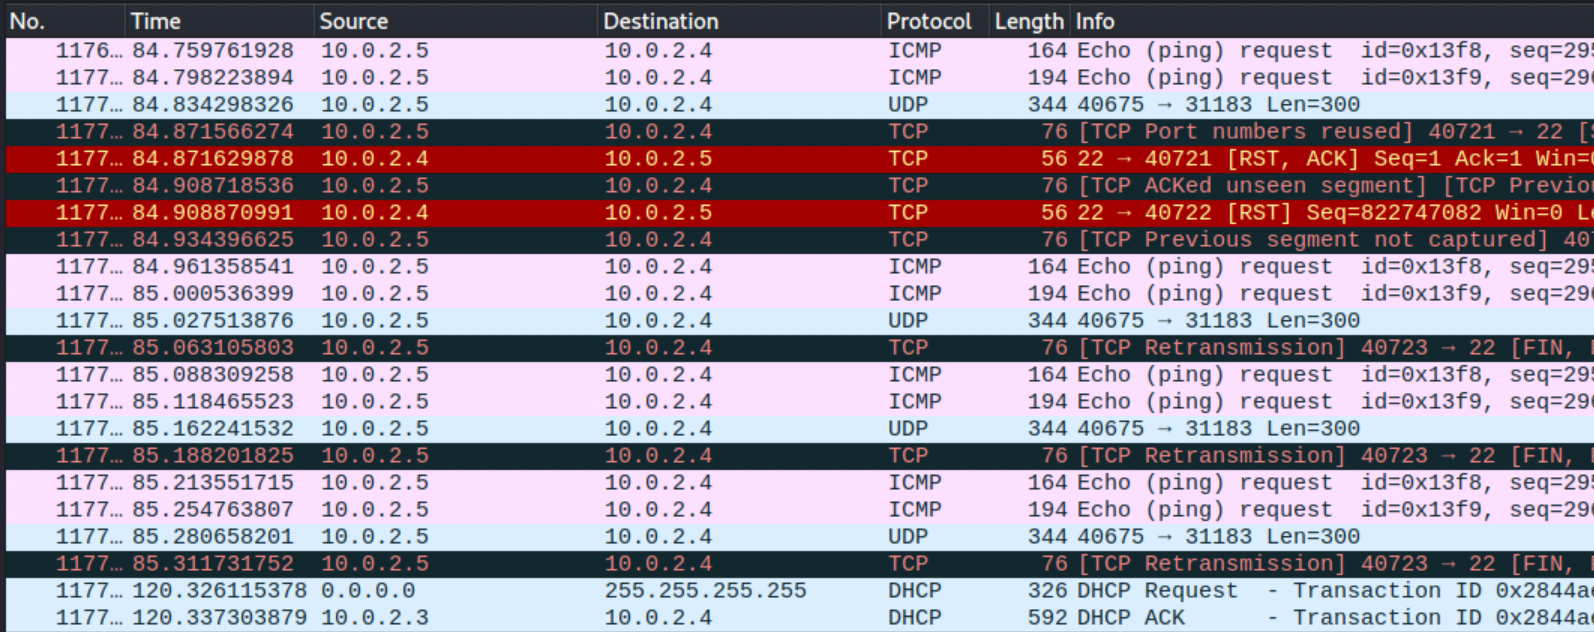
\includegraphics[width=\linewidth]{img/ws_firewall_standard_2.png}
	\caption{Fort.: Datenverkehr der Opfermaschine}
	\label{fig:ws_firewall_standard_2}
\end{figure}

\subsubsection{nmap 10.0.2.4 -sU -T4}
Im Script wurde der Port 53, welcher für das DNS Protokoll verwendet wird, für ausgehende UDP Pakete geöffnet. Diese Ausnahmeregelung ist die Einzige, die UDP betrifft. Da die Ausnahme nur für ausgehende Pakete gilt, ist es zu erwarten, dass ähnlich wie in Kapitel 2.2.2 alle Ports als ``open | filtered`` gezeigt werden. \\
Output: 

\lstinputlisting{scripts/scans/nmap_sU_T4_standard}
\begin{figure}
	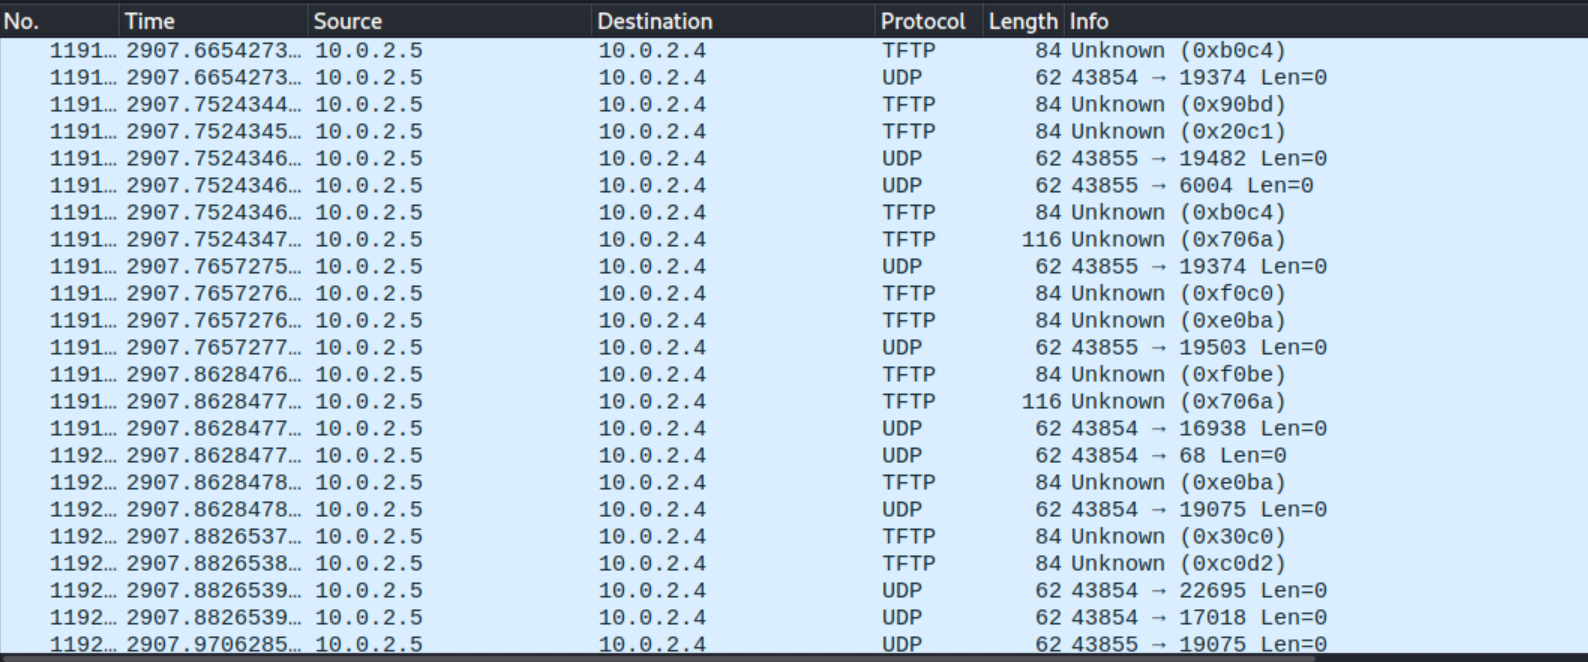
\includegraphics[width=\linewidth]{img/ws_firewall_standard_udp.png}
	\caption{Datenverkehr der Opfermaschine – UDP}
	\label{fig:ws_firewall_standard_udp}
\end{figure}
\subsection{Penetrationtest – Outward}

Abschließend wird auch bei dieser Firewall-Konfiguration überprüft, welchen Einfluss die Firewall auf die ausgehenden Verbindungen der Maschine besitzt. Das Verfahren ist gleich dem der zwei Vorgängern. 

\subsubsection*{wget https://google.com}
Zunächst soll getestet werden, ob google.com erreichbar ist. Die Ports für http und https sind beide in die ausgehende Richtung freigegeben, demnach sollte es zu erwarten sein, dass eine Verbindung zum WWW hergestellt werden kann. Zusätzlich wurde der Port 53 für DNS freigegeben. So sollte es möglich sein über die Domain google.com eine Verbindung aufzubauen. 
\begin{figure}
	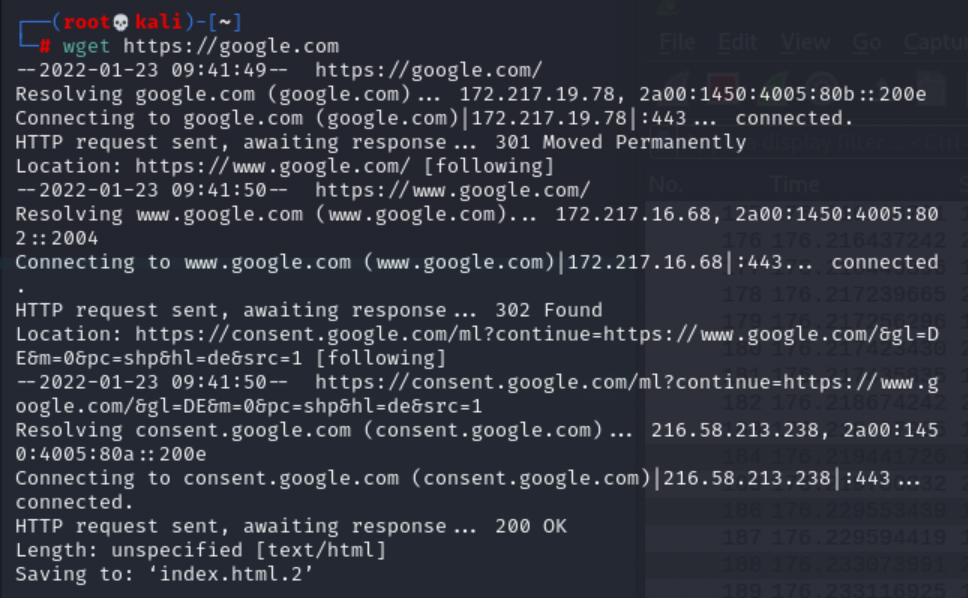
\includegraphics[width=\linewidth]{img/standard_in_out_output.png}
	\caption{Erfolgreicher Verbindungsaufbau zum WWW bei Standardfirewall}
	\label{fig:standard_in_out}
\end{figure}

Wie im Output \ref{fig:standard_in_out} zu erkennen, lässt sich sowohl die Domain google.com auflösen, wie auch eine Verbindung zu der Gleichen herstellen. Dies lässt darauf schließen dass die freigegeben Ports ordnungsgemäß funktionieren, obwohl sie nur in eine "Richtung" freigegeben sind. Dies funktioniert, da established connections – also etablierte Verbindungen – freigegeben sind. Das bedeutet dass Antworten auf die Anfragen der Maschine durch die Firewall kommen aber fremde Anfragen nicht. Dies hilft dabei ungewünschte Verbindungen vorzubeugen.

\subsubsection*{nc 10.0.2.5 4445}
Abschließend soll nun getestet werden, ob die Maschine eine Verbindung zu ihrem Nachbarn über arbiträre Ports aufbauen kann. Dafür wird erneut mittels des NetCat Befehls versucht eine Verbindung zur Maschine auf 10.0.2.5 aufzubauen. 
Der Befehl auf dieser Nachbarmaschine ist gleich dem der anderen Tests aus Kapiteln 2.1.3 und 2.2.3. Genau so ist der Befehl auf der Maschine 10.0.2.4 gleich. Da bis auf ein paar Ausnahmen alle Ports weiterhin von der Firewall geblockt werden, ist es anzunehmen das dieser Verbindungsaufbau fehlschlagen wird. Es wird wieder ein Timeout von 60 Sekunden eingestellt. 

\lstinputlisting{scripts/nc_closed}

Wie zu erkennen ist es erneut fehlgeschlagen eine Verbindung zur Nachbarmaschine aufzubauen. 
